\section{Exercise1}

This exercise investigates how the parameterization of a student neural
network relative to a teacher network affects its ability to learn.

\subsection{Setup}

We instantiate the teacher model $T$ as a fully connected neural network,
mapping a 100-dimensional input to a single output scalar, with three hidden
layers of 75, 50, 10 neurons respectively. 
We then instantiate three student models $S_1, S_2, S_3$ as fully connected neural
networks with the following architectures:
\begin{align*}
    S_1 &\text{ : 100-10-1}
    \\
    S_2 &\text{ : 100-75-50-10-1}
    \\
    S_3 &\text{ : 100-200-200-200-100-1}
\end{align*}
After doing so with proceed by generating
the testing data by sampling from the teacher model.
\begin{align*}
    D_{test} &= \{(x_i, T(x_i))\}_{i=1}^{N}
    \\
    x_i &\sim \mathcal{U}(0, 2)^{100}
    \\
    N &= 6 \cdot 10^4
\end{align*}
Conversely, the training data is generated lazily by sampling from the teacher
during training. 


\subsection{Training}
We train each model with the Adam optimizer for 1000 steps with a batch size of
128. We use the mean squared error loss function and the learning rate is tuned
by empirical validation as suggested in class. The learning rate for each model is as follows:
\begin{align*}
    S_1 &\text{ : 2e-1}
    \\
    S_2 &\text{ : 3.5e-2}
    \\
    S_3 &\text{ : 9e-3}
\end{align*}

The loss evolution plots are reported below.
\begin{figure}[H]
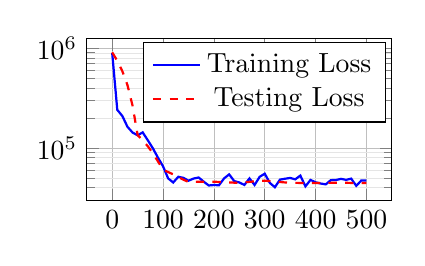
\begin{tikzpicture}
    \begin{axis}[
        width=0.45\textwidth,
        height=0.3\textwidth,
        % xlabel={Epochs},
        % ylabel={Loss},
        % Y logarithmic axis
        ymode=log,
        grid=both,
        grid style={line width=.1pt, draw=gray!20},
        major grid style={line width=.2pt,draw=gray!50},
    ]

    % Training Loss
    \addplot[color=blue, thick] table[row sep=\\] {
            Epoch Loss \\
            0 894546.0125 \\
            10 240647.390625 \\
            20 208289.765625 \\
            30 162688.459375 \\
            40 142362.18125 \\
            50 133538.4703125 \\
            60 142785.1875 \\
            70 119116.9234375 \\
            80 98903.753125 \\
            90 79687.421875 \\
            100 65185.97109375 \\
            110 49347.9375 \\
            120 44863.6984375 \\
            130 51181.3390625 \\
            140 49958.3921875 \\
            150 46749.040625 \\
            160 49113.27734375 \\
            170 50369.7625 \\
            180 45679.73125 \\
            190 41866.0859375 \\
            200 42301.59765625 \\
            210 42076.32109375 \\
            220 49279.109375 \\
            230 54109.38828125 \\
            240 46322.3109375 \\
            250 44875.58515625 \\
            260 42411.8765625 \\
            270 49259.47734375 \\
            280 42368.46875 \\
            290 51127.92109375 \\
            300 54962.2125 \\
            310 44441.3359375 \\
            320 40187.79453125 \\
            330 47953.93203125 \\
            340 48932.9765625 \\
            350 49824.9890625 \\
            360 48233.25390625 \\
            370 52632.85078125 \\
            380 41030.32734375 \\
            390 47593.34453125 \\
            400 45065.97109375 \\
            410 43793.12265625 \\
            420 42970.01953125 \\
            430 47376.1078125 \\
            440 47519.26484375 \\
            450 48781.07734375 \\
            460 47663.4484375 \\
            470 49045.4625 \\
            480 41527.11328125 \\
            490 47051.859375 \\
            500 47051.859375 \\
    };
    \addlegendentry{Training Loss}

    % Testing Loss
    \addplot[color=red, thick, dashed] table[row sep=\\] {
            Epoch Loss \\
            0 907952.7412288137 \\
            10 747379.7047881356 \\
            20 586806.6683474575 \\
            30 426233.6319067796 \\
            40 265660.59546610166 \\
            50 134148.47342955507 \\
            60 118880.00900953388 \\
            70 103611.5445895127 \\
            80 88343.08016949151 \\
            90 73074.61574947034 \\
            100 60242.12152542373 \\
            110 57153.50808527542 \\
            120 54064.89464512712 \\
            130 50976.28120497881 \\
            140 47887.667764830505 \\
            150 45428.732682733054 \\
            160 45488.51103283898 \\
            170 45548.28938294492 \\
            180 45608.06773305085 \\
            190 45667.84608315678 \\
            200 45666.05669226695 \\
            210 45417.99633739407 \\
            220 45169.93598252119 \\
            230 44921.8756276483 \\
            240 44673.81527277542 \\
            250 44570.649472987294 \\
            260 45047.061893538135 \\
            270 45523.47431408898 \\
            280 45999.88673463983 \\
            290 46476.299155190674 \\
            300 46765.07284427966 \\
            310 46303.29160752118 \\
            320 45841.51037076271 \\
            330 45379.72913400424 \\
            340 44917.94789724576 \\
            350 44537.04123411017 \\
            360 44479.6328654661 \\
            370 44422.22449682203 \\
            380 44364.81612817797 \\
            390 44307.4077595339 \\
            400 44275.25231726695 \\
            410 44344.10858050848 \\
            420 44412.96484375 \\
            430 44481.82110699153 \\
            440 44550.67737023305 \\
            450 44589.44007415255 \\
            460 44507.8285407839 \\
            470 44426.21700741526 \\
            480 44344.60547404661 \\
            490 44262.99394067797 \\
            500 44262.99394067797 \\
    };
    \addlegendentry{Testing Loss}
        
    \pgfplotsset{xtick={0,100,200,300,400,500}}

    \end{axis}
\end{tikzpicture}
\end{figure}



\begin{figure}[H]
    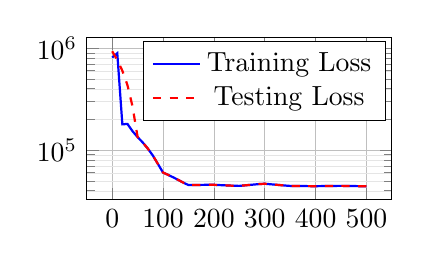
\begin{tikzpicture}
        \begin{axis}[
            width=0.45\textwidth,
            height=0.3\textwidth,
            % xlabel={Epochs},
            % ylabel={Loss},
            % Y logarithmic axis
            ymode=log,
            grid=both,
            grid style={line width=.1pt, draw=gray!20},
            major grid style={line width=.2pt,draw=gray!50},
        ]
    
        % Training Loss
    \addplot[color=blue, thick] table[row sep=\\] {
        Epoch Loss \\
        0 808947.237500 \\
        10 890469.778125 \\
        20 178986.278125 \\
        30 180629.865625 \\
        40 153239.050000 \\
        50 134148.473430 \\
        60 118880.009010 \\
        70 103611.544590 \\
        80 88343.080169 \\
        90 73074.615749 \\
        100 60242.121525 \\
        110 57153.508085 \\
        120 54064.894645 \\
        130 50976.281205 \\
        140 47887.667765 \\
        150 45428.732683 \\
        160 45488.511033 \\
        170 45548.289383 \\
        180 45608.067733 \\
        190 45667.846083 \\
        200 45666.056692 \\
        210 45417.996337 \\
        220 45169.935983 \\
        230 44921.875628 \\
        240 44673.815273 \\
        250 44570.649473 \\
        260 45047.061894 \\
        270 45523.474314 \\
        280 45999.886735 \\
        290 46476.299155 \\
        300 46765.072844 \\
        310 46303.291608 \\
        320 45841.510371 \\
        330 45379.729134 \\
        340 44917.947897 \\
        350 44537.041234 \\
        360 44479.632865 \\
        370 44422.224497 \\
        380 44364.816128 \\
        390 44307.407760 \\
        400 44275.252317 \\
        410 44344.108581 \\
        420 44412.964844 \\
        430 44481.821107 \\
        440 44550.677370 \\
        450 44589.440074 \\
        460 44507.828541 \\
        470 44426.217007 \\
        480 44344.605474 \\
        490 44262.993941 \\
        500 44262.993941 \\
};
\addlegendentry{Training Loss}

% Testing Loss
\addplot[color=red, thick, dashed] table[row sep=\\] {
        Epoch Loss \\
        0 931903.038363 \\
        10 765993.065985 \\
        20 600083.093607 \\
        30 434173.121229 \\
        40 268263.148851 \\
        50 134148.473430 \\
        60 118880.009010 \\
        70 103611.544590 \\
        80 88343.080169 \\
        90 73074.615749 \\
        100 60242.121525 \\
        110 57153.508085 \\
        120 54064.894645 \\
        130 50976.281205 \\
        140 47887.667765 \\
        150 45428.732683 \\
        160 45488.511033 \\
        170 45548.289383 \\
        180 45608.067733 \\
        190 45667.846083 \\
        200 45666.056692 \\
        210 45417.996337 \\
        220 45169.935983 \\
        230 44921.875628 \\
        240 44673.815273 \\
        250 44570.649473 \\
        260 45047.061894 \\
        270 45523.474314 \\
        280 45999.886735 \\
        290 46476.299155 \\
        300 46765.072844 \\
        310 46303.291608 \\
        320 45841.510371 \\
        330 45379.729134 \\
        340 44917.947897 \\
        350 44537.041234 \\
        360 44479.632865 \\
        370 44422.224497 \\
        380 44364.816128 \\
        390 44307.407760 \\
        400 44275.252317 \\
        410 44344.108581 \\
        420 44412.964844 \\
        430 44481.821107 \\
        440 44550.677370 \\
        450 44589.440074 \\
        460 44507.828541 \\
        470 44426.217007 \\
        480 44344.605474 \\
        490 44262.993941 \\
        500 44262.993941 \\
};
\addlegendentry{Testing Loss}
            
        \pgfplotsset{xtick={0,100,200,300,400,500}}
    
        \end{axis}
    \end{tikzpicture}
    \end{figure}
    
    
    
\input{content/plots/loss_over.tex} 

The x-axis has been truncated to 500 steps because the loss evolution of the
student models was not evolving much after that point. Hereafter we report the final
loss achieved by each model.

\begin{table}[H]
    \centering
    \begin{tabular}{c|cc}
        \toprule
        \textbf{Model} & Train Loss & Test Loss \\
        \midrule
        $S_1$ & 47755 & 44895 \\
        $S_2$ & \textbf{42176} & 54148 \\
        $S_3$ & 47430 & \textbf{42891} \\
        \bottomrule
    \end{tabular}
\end{table}

The best on-sample performance is achieved by the $S_2$ model,
which shares the same architecture as the teacher model. However,
when evaluating out-of-sample performance, the $S_3$ model, the over-parameterized 
one, exhibits the lowest estimated generalization error. Interestingly,
the worst-performing model among the three is $S_2$, the equally parameterized version,
while even the under-parameterized model, $S_1$, outperforms it. \\

This behavior can be explained by the double descent phenomenon,
where model performance initially improves as complexity increases,
deteriorates at the interpolation threshold, and then improves again
with further complexity. The three models, in this case, perfectly 
reproduce the three regime described in literature
\cite{belkin2019biasvariance} \cite{nakkiran2019deepdoubledescent} \cite{lafon2024doubledescent}
, which we briefly summarize below.
\begin{itemize}
    \item \textbf{Under-parameterized regime}: the model is too simple to capture the complexity of the data.
    \item \textbf{Interpolation threshold}: the model is complex enough to interpolate the data, but not to generalize.
    \item \textbf{Over-parameterized regime}: the model is complex enough to generalize.
\end{itemize}


\subsection{Weights distribution}

We now analyze the distribution of the weights of the student models,
both network-wide and layer-wise.

\begin{figure}[H]
    \centering
    \includegraphics[width=0.45\textwidth]{figures/weights_distribution.png}
    \caption{Weights distribution for the student models.}
\end{figure}
\begin{figure}[H]
    \centering
    \begin{tabular}{c|cc}
    \toprule
    \textbf{Model}                      & Mean & Std \\
    \midrule
    $S_1$                                 & -0.98         & 2.39         \\
    $S_2$                                 & -0.10         & 0.42         \\
    $S_3$                                 & -0.01         & 0.11         \\
    $T$                                   &  0.00         & 0.99         \\
    \bottomrule
    \end{tabular}
    \caption{Summary statistics for students and teacher models.}
\end{figure}

As we can see, the model closest in mean to the teacher is the over-parameterized
one, which is also the one with the lowest variance. The under-parameterized model, 
instead, has the highest variance and the lowest mean. \\
Means and standard deviations for each layer are reported in
the table below.

\begin{table}[H]
    \centering
    \begin{tabular}{c|cc|cc|cc|cc}
    \toprule
    \textbf{Layer} & $\mathbf{\mu_1}$ & $\mathbf{\sigma_1}$ & $\mathbf{\mu_2}$ & $\mathbf{\sigma_2}$ & $\mathbf{\mu_3}$ & $\mathbf{\sigma_3}$ & $\mathbf{\mu_T}$ & $\mathbf{\sigma_T}$ \\
    \midrule
    $w_1$ & -0.98 & 2.39 & -0.13 & 0.50 & -0.03 & 0.14 & 0.00 & 0.99 \\
    $b_1$ & -0.51 & 2.11 & -0.04 & 0.31 & -0.01 & 0.05 & -0.12 & 0.82 \\
    $w_2$ & -1.32 & 2.34 & -0.06 & 0.27 & -0.01 & 0.10 & 0.01 & 0.99 \\
    $b_2$ & -7.27 & 0.00 & 0.02 & 0.40 & 0.02 & 0.11 & 0.00 & 0.93 \\
    $w_3$ & - & - & -0.06 & 0.25 & -0.01 & 0.09 & -0.02 & 1.02 \\
    $b_3$ & - & - & 0.14 & 0.46 & 0.04 & 0.11 & -0.11 & 0.99 \\
    $w_4$ & - & - & -0.02 & 0.34 & -0.01 & 0.10 & -0.12 & 0.91 \\
    $b_4$ & - & - & -0.61 & 0.00 & 0.00 & 0.14 & 0.78 & 0.00 \\
    $w_5$ & - & - & - & - & 0.00 & 0.14 & - & - \\
    $b_5$ & - & - & - & - & -0.11 & 0.14 & - & - \\
    \bottomrule
    \end{tabular}
\end{table}

As we can see, the over-parameterized model has the weights more similarly distributed
across layers, with the under-parameterized model having the most different distributions.
Moreover if we compute the network-wide norm and the layer-wise norms we can see that the
over-parameterized model has the lowest norm on average.

\begin{table}[H]
    \centering
    \begin{tabular}{c|ccc|c}
    \toprule
    \textbf{Layer} & $S_1$ & $S_2$ & $S_3$ & $T$ \\
    \midrule
    $w_1$ & 81.67 & 44.82 & 20.22 & 85.37 \\
    $b_1$ & 6.88  & 2.71  & 0.79  & 7.14  \\
    $w_2$ & 8.49  & 16.89 & 20.37 & 60.67 \\
    $b_2$ & 7.27  & 2.84  & 1.56  & 6.55  \\
    $w_3$ & -     & 9.10  & 18.66 & 36.10 \\
    $b_3$ & -     & 2.39  & 1.63  & 5.00  \\
    $w_4$ & -     & 1.68  & 14.56 & 4.61  \\
    $b_4$ & -     & 0.61  & 0.93  & 0.78  \\
    $w_5$ & -     & -     & 1.39  & -     \\
    $b_5$ & -     & -     & 0.11  & -     \\
    \bottomrule
    \end{tabular}
\end{table}
